\section{Gestione amministrativa della revisione}
\subsection{Comunicazione e risoluzione di anomalie}
Un'anomalia corrisponde a:
\begin{itemize}
	\item Violazione delle norme tipografiche da parte di un documento.
	\item Incongruenza del prodotto con funzionalità indicate nell'analisi dei requisiti.
\end{itemize}
Nel caso in cui un Verificatore o un membro del gruppo individui un anomalia dovrà segnalarlo aprendo un ticket$_G$ nella forma descritta nella sezione 5.2 delle Norme di Progetto. Un verificatore ha il compito di controllare le pull request quindi nel caso trovasse un anomalia deve bloccare la pull specificando il motivo al richiedente come descritto nella sezione 5.4 delle Norme di Progetto.
\subsection{Trattamento delle discrepanze}
Una discrepanza è un discostamento dai requisiti attesi del capitolato o una violazione delle Norme di Progetto.
Il trattamento delle discrepanze avviene come la gestione delle anomalie. Quando un membro del gruppo o il Verificatore ne individuasse una segnalerà il problema aprendo un ticket oppure un Verificatore può bloccare la pull specificando il motivo al richiedente come per il trattamento delle anomalie.
\subsection{Procedure di controllo di qualità di processo}
Le Procedure di controllo di qualità di processo si basano sul ciclo di Deming o PDCA$_G$. Questo garantisce un miglioramento continuo di tutti i processi e delle attività di verifica che si realizza con comunicazioni attive delle componenti del gruppo e con la connessione delle fasi di analisi, progettazione, verifica e collaudo.
La qualità dei processi viene monitorata anche grazie alla qualità di prodotto perchè un prodotto di bassa qualità può indicare che uno o più processi vadano migliorati. Per questo motivo si presta attenzione a monitorare i singoli processi ed è necessario quindi che i processi vengano pianificati nel dettaglio, le risorse vengano ripartite nella pianificazione in modo chiaro e ci sia un adeguato controllo sui processi.
\begin{figure}[h!]
		\centering
		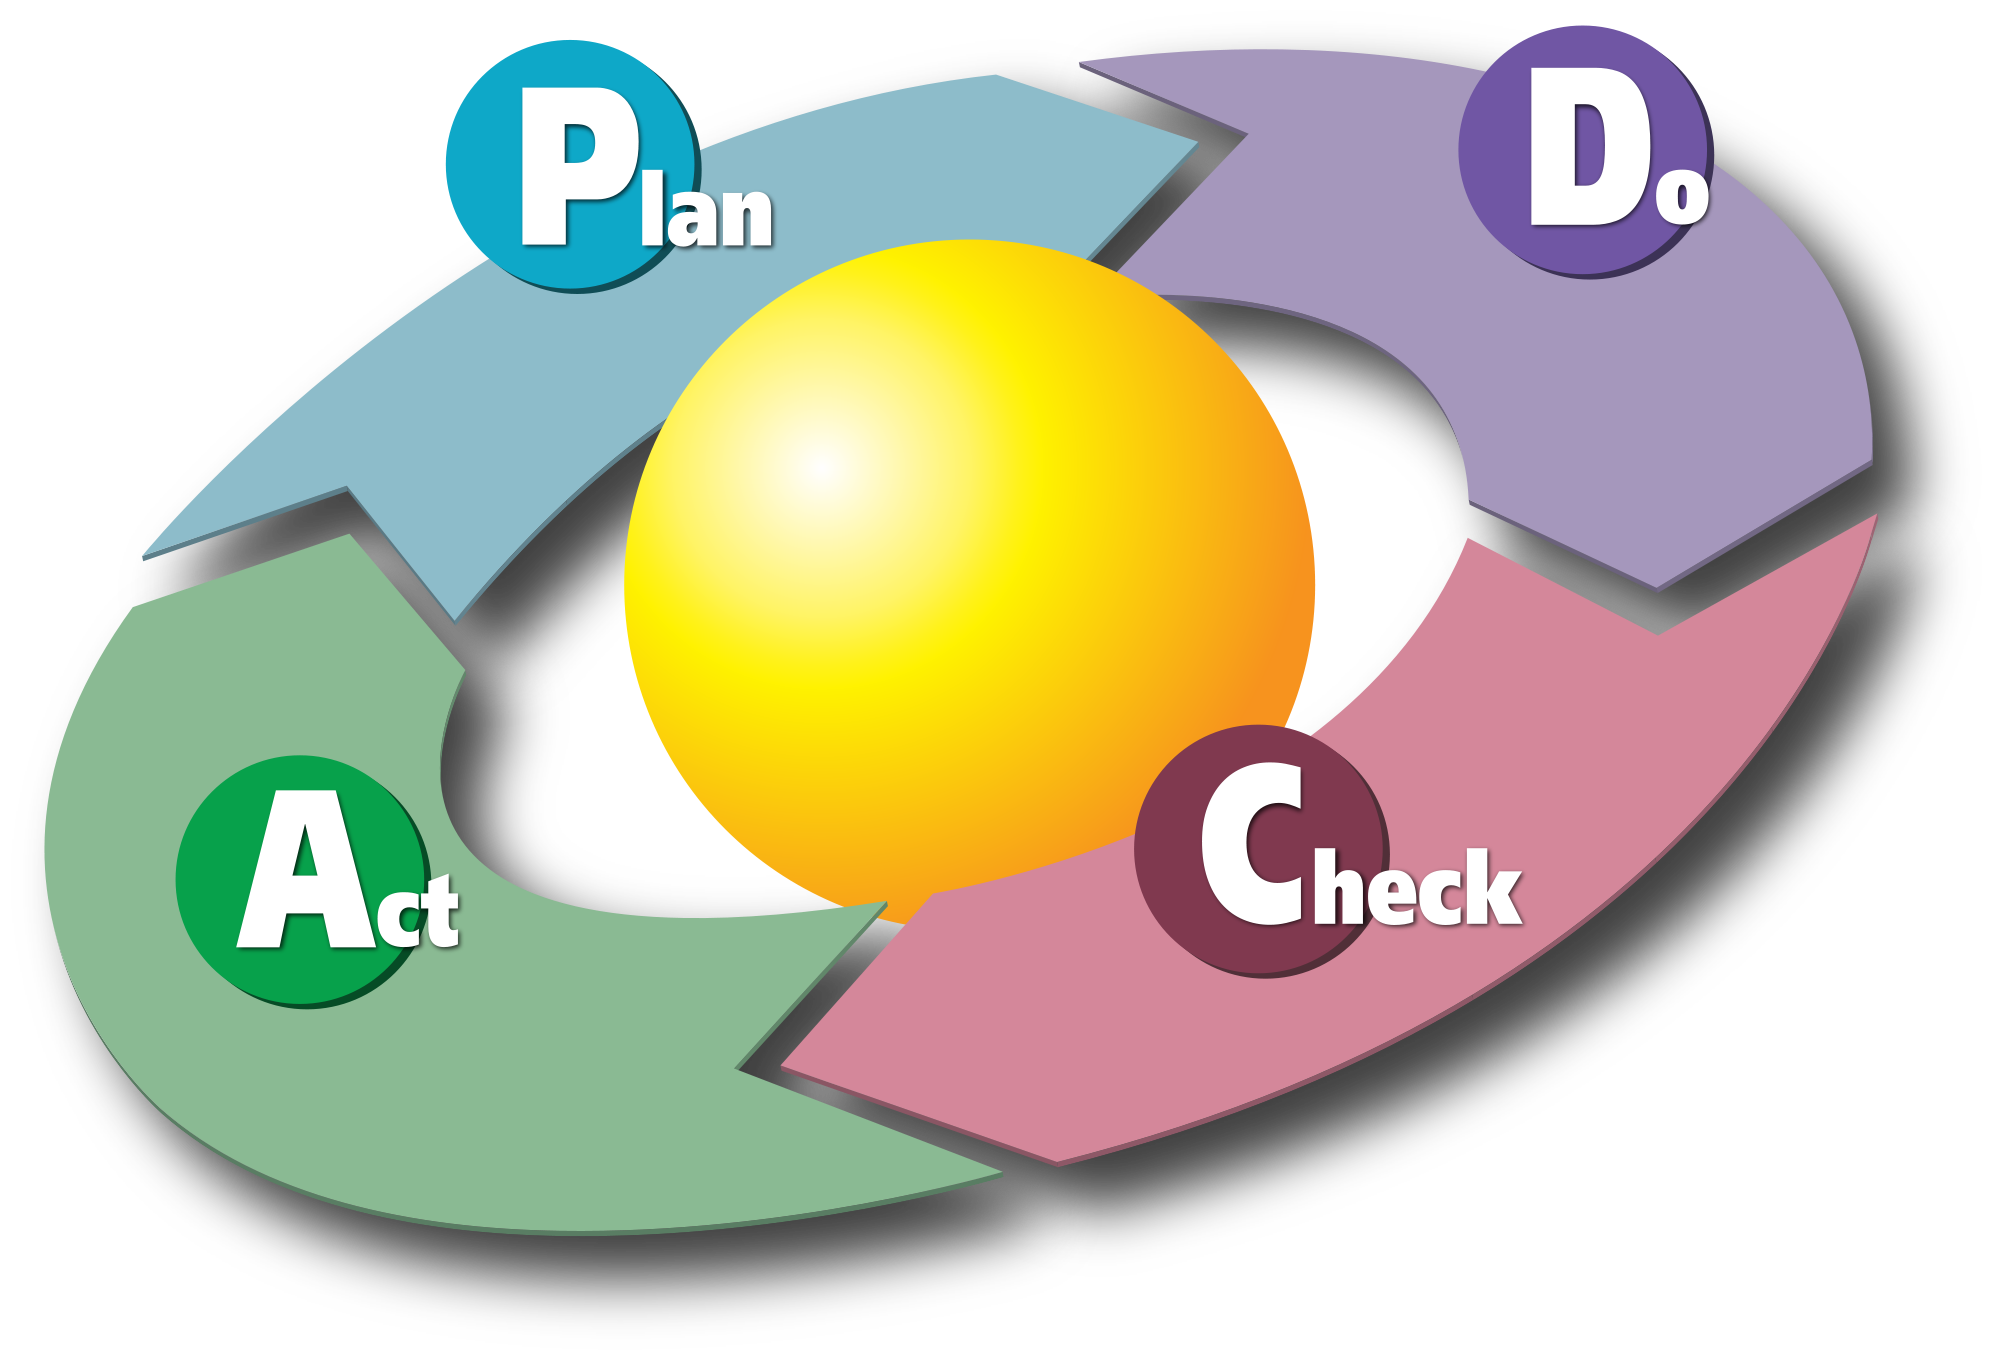
\includegraphics[scale=.6]{img/2000px-PDCA_Cycle.svg.png}
		\caption{Modello PDCA}
		\label{fig:ModelloSpy}
\end{figure}